\secrel{Создание проекта в менеджере проектов \prog{kicad}}

В верхней части панели \term{менеджера проектов} \prog{kicad}
имеются большие кнопки запуска компонентов KiCad:

% \begin{itemize}
% \item \icoesch\ \prog{EeSchema}\ --- Редактор принципиальных схем
% \item
% 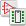
\includegraphics[height=0.1\textheight]{kicad/icon_cvpcb.png}\
% \prog{CvPcb}\
% --- Программа редактирования падстеков (отверстий и площадок)
% \item
% 
\includegraphics[height=0.1\textheight]{kicad/icon_pcbnew.png}
% \prog{Pcbnew}\ ---
% Редактор печатных плат
% \item
% 
\includegraphics[height=0.1\textheight]{kicad/icon_gerbview.png}
% \prog{GerbView}\ --- Программа просмотра фотошаблонов в формате Gerber
% \item \prog{Bitmap2Component}\ --- Создание компонента из черно-белого
% изображения (например логотипа)
% \item
% 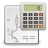
\includegraphics[height=0.1\textheight]{kicad/icon_pcbcalculator.png}
% \prog{PcbCalculator}\ --- Калькулятор для печатных плат
% \item
% 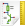
\includegraphics[height=0.1\textheight]{kicad/icon_pagelayout.png}
% \prog{PageLayout}\ --- редактор формата листа схемы
% \end{itemize}

Каждая кнопка запускает соответствующую программу. Мы будем использовать эти
программы по мере изучения.

\bigskip
Лучше всего для каждого проекта использовать раздельные папки; в противном
случае система может сбиться с толку, если файлы из разных проектов будут лежать
в одной папке. Проделайте следующие шаги:

% \begin{enumerate}
%   \item Создайте папку проекта \file{D:/ARM/SpindleDriver}
%   \item Запустите программу KiCad
%   \item Создайте проект (project)
%   \begin{itemize}
%     \item 
% На панели инструментов KiCad выберите левую иконку с подсказкой\\
% \menu{Начать новый проект}, используйте команду меню
% \menu{Файл>Новый>Пустой} или сочетание клавиш \keys{Ctrl+N}.
%     \item 
% В диалоге \menu{Создать новый проект} выберите созданную папку
% выберите только что созданную папку \file{D:/ARM/SpindleDriver} и
% введите имя проекта \menu{\file{SpindleDriver}} и нажмите \menu{Сохранить}.
% 	\item
% Если папка проекта содержит какие-то файлы, будет выведено окно выбора:
% создать подпапку с именем проекта \menu{Yes}, или записать файл проекта
% в указанную папку как есть \menu{No}. Нажмите No.
%     \item 
% Сохраните проект кнопкой \menu{Сохранить текущий проект}, \menu{Файл>Сохранить}
% или \keys{Ctrl+S}.
% 	\item
% В папке появится файл \file{SpindleDriver.pro}, содержащий установки вашего 
% проекта. Файл имеет тектовый формат, поэтому при необходимости его можно открыть
% в любом редакторе и вручную аккуратно подправить, например скорректировать
% настройки зазоров печатной платы.
%   \end{itemize}
% \end{enumerate}

\secrel{Создание принципиальной схемы в \prog{eeschema}\ (часть 1)}

Запустите редактор принципиальных схем, нажав на панели KiCad большую кнопку
\icoesch.

% При первом запуске \prog{eeschema}\ стартует с новым проектом и
% показывает предупреждение, что файла схемы еще нет. Просто нажмите \menu{ОК}.

% Если вас не устраивает черный фон рабочец области или цвета элементов схемы,
% поменяйте настроки цветов \menu{Настройки>Цвета}.
% 
% На правом краю окна редактора схем есть вертикальная панель инструментов,
% которые мы и будем использовать для рисования схемы. Этими инструментами можно
% выбирать объекты, размещать компоненты, вводить связи и т.д.
% 
% 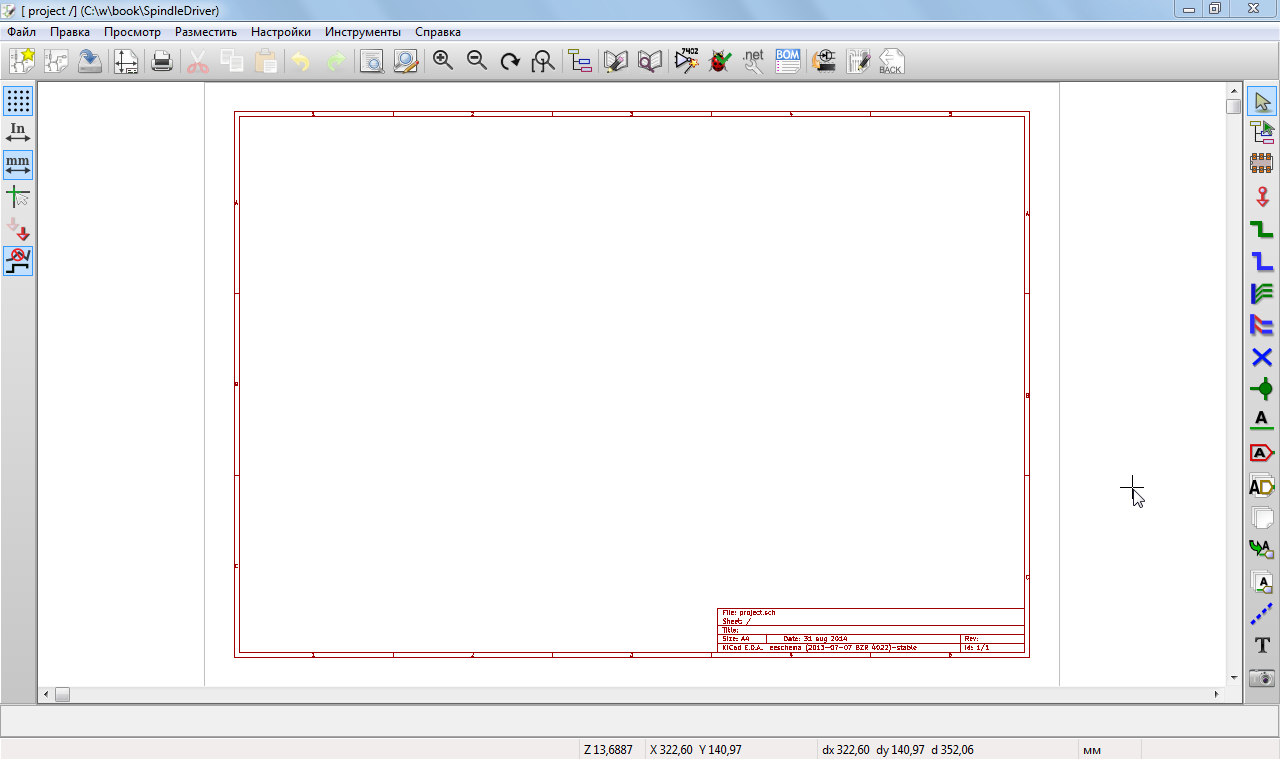
\includegraphics[width=0.9\textwidth]{kicad/ee15.png}
% 
% Завершение работы инструмента: вы можете выбрать другой инструмент из правой
% инструментальной панели или же указать \menu{Отложить инструмент} по правому
% клику мышки \keys{\rms}.

\secrel{Инструмент \emph{Добавить компоненты}}

% \begin{itemize}
%   \item 
% На правой панели нажмите кнопку \menu{Разместить компонент}\
% 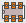
\includegraphics[height=2em]{kicad/ee21.png}. Курсор изменится со стрелки на
% карандаш. Удобнее использовать сочетание клавиш \keys{Shift+A}.
% Кликните в поле схемы чтобы начать размещение компонента. Появится диалог
% \menu{Выбор компонента}. Вы можете выбрать компонент несколькими путями:
%   \item
%   \begin{enumerate}
%     \item 
% Если вы знаете точное имя копонента, введите его в поле \menu{Имя}, а
% затем нажмите \keys{Enter} или \keys{OK}.
%     \item 
% Если вы знаете имя только приблизительно, в поле \menu{Имя} введите шаблон для
% поиска, например, \menu{*BD*}, затем нажмите \keys{Enter} или \keys{OK}. Вы
% увидите окно \\\menu{Выбрать компонент} со списком найденных компонентов.
% 
% 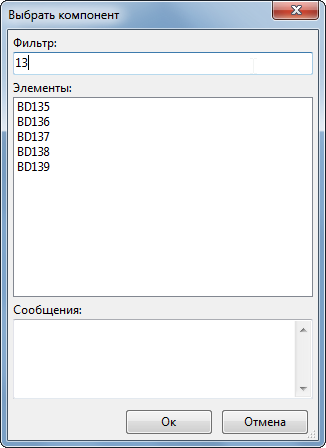
\includegraphics[height=0.5\textheight]{kicad/ee16.png}
%     \item 
% Вы можете искать компонент по ключевому слову, введя его в поле \menu{Имя},
% затем кликнув \menu{Поиск по ключевому слову}. Однако на данный момент качество
% библиотек все еще низкое, и немногие компоненты имеют ключевые слова, поэтому
% эта возможность полезна косвенно.
%     \item 
% Можно выбрать недавно использованные компоненты из \menu{Списка истории}.
%     \item 
% Кнопка \menu{Список всех} вызывает диалог, в котором можно выбрать сначала
% библиотеку \menu{74xx}, а затем ее компонент \menu{74HCT04}.
%     \item 
% Кнопка \menu{Выбор просмотром} вызывает \menu{Обзор библиотек}, позволяя
% просмотреть библиотеки и находящиеся в них условные графические изображения.
% 
% 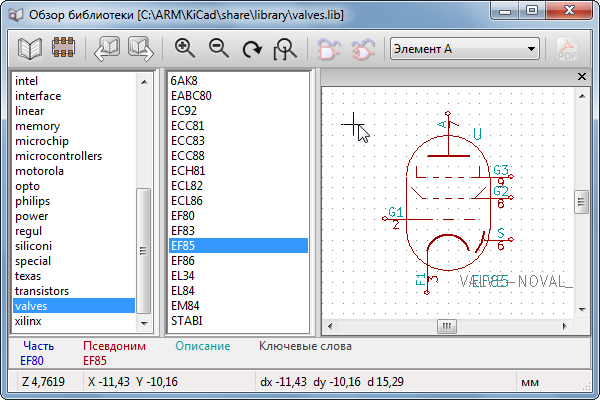
\includegraphics[height=0.5\textheight]{kicad/ee19.png}
% 
%   \end{enumerate} 
% \end{itemize}
% 
% Вы также можете
% вызвать обозреватель библиотек кнопкой\\
% \menu{Просмотр библиотек и
% компонентов}\ 
\includegraphics[height=2em]{kicad/ee20.png}
% 
% Выбрав элемент \dblms, вставьте символ в нужное место схемы \lms.
% Позже вы сможете переместить его если нужно.
% Зеркальное отражение компонента можно произвести следующим образом:
% 
% \begin{itemize}
%   \item Поместите курсор на компоненте.
%   \item По \rms\ выберите \menu{Ориентация компонента>Отражение}. 
%   \item Без использования \term{контекстного меню}\ --- наведите мышь на
%   компонент и нажмите кнопку \keys{X}\ или \keys{Y}.
% \end{itemize}
% 
